\documentclass[tikz,border=1mm]{standalone}
% Shared publication styles; labels designed for 170 mm inclusion width.
\usepackage[T1]{fontenc}
\usepackage{lmodern}
\usepackage{amsmath}
\usepackage{tikz}
\usepackage{pgfplots}
\pgfplotsset{compat=1.18}
\usetikzlibrary{arrows.meta,positioning,calc,fit,backgrounds,shapes.geometric,patterns,decorations.pathreplacing,circuits.logic.US}
\definecolor{ink}{HTML}{263238}
\definecolor{muted}{HTML}{60717D}
\definecolor{grid}{HTML}{DCE5EA}
\definecolor{normal}{HTML}{4C78A8}
\definecolor{compact}{HTML}{59A14F}
\definecolor{june}{HTML}{8A6BBE}
\definecolor{warn}{HTML}{C18523}
\definecolor{bad}{HTML}{BC514C}
\definecolor{phasezero}{HTML}{DBEAF8}
\definecolor{phaseone}{HTML}{DFEFD9}
\definecolor{phasetwo}{HTML}{FFF1C8}
\definecolor{phasethree}{HTML}{ECE1F6}
\tikzset{
  every picture/.style={font=\sffamily\fontsize{8}{9.5}\selectfont,text=ink},
  >=Latex,
  box/.style={draw=ink!60,fill=white,rounded corners=1.2pt,align=center,inner sep=4pt,line width=.55pt},
  flow/.style={-{Latex[length=1.7mm,width=1.2mm]},draw=ink,line width=.65pt},
  control/.style={flow,dashed,draw=muted},
  retry/.style={flow,draw=warn},
  paneltitle/.style={font=\sffamily\bfseries\fontsize{9}{10.5}\selectfont,anchor=west},
  smallnote/.style={font=\sffamily\fontsize{7}{8.5}\selectfont,text=muted,align=left},
  gridline/.style={draw=grid,line width=.2pt},
}
\pgfplotsset{every axis/.append style={
  font=\sffamily\fontsize{8}{9.5}\selectfont,
  label style={font=\sffamily\fontsize{8}{9.5}\selectfont},
  tick label style={font=\sffamily\fontsize{7.5}{9}\selectfont},
  legend style={font=\sffamily\fontsize{7.5}{9}\selectfont,draw=none,fill=none},
  axis line style={draw=ink!65},tick style={draw=ink!65},
  grid style={draw=grid},
}}

\begin{document}
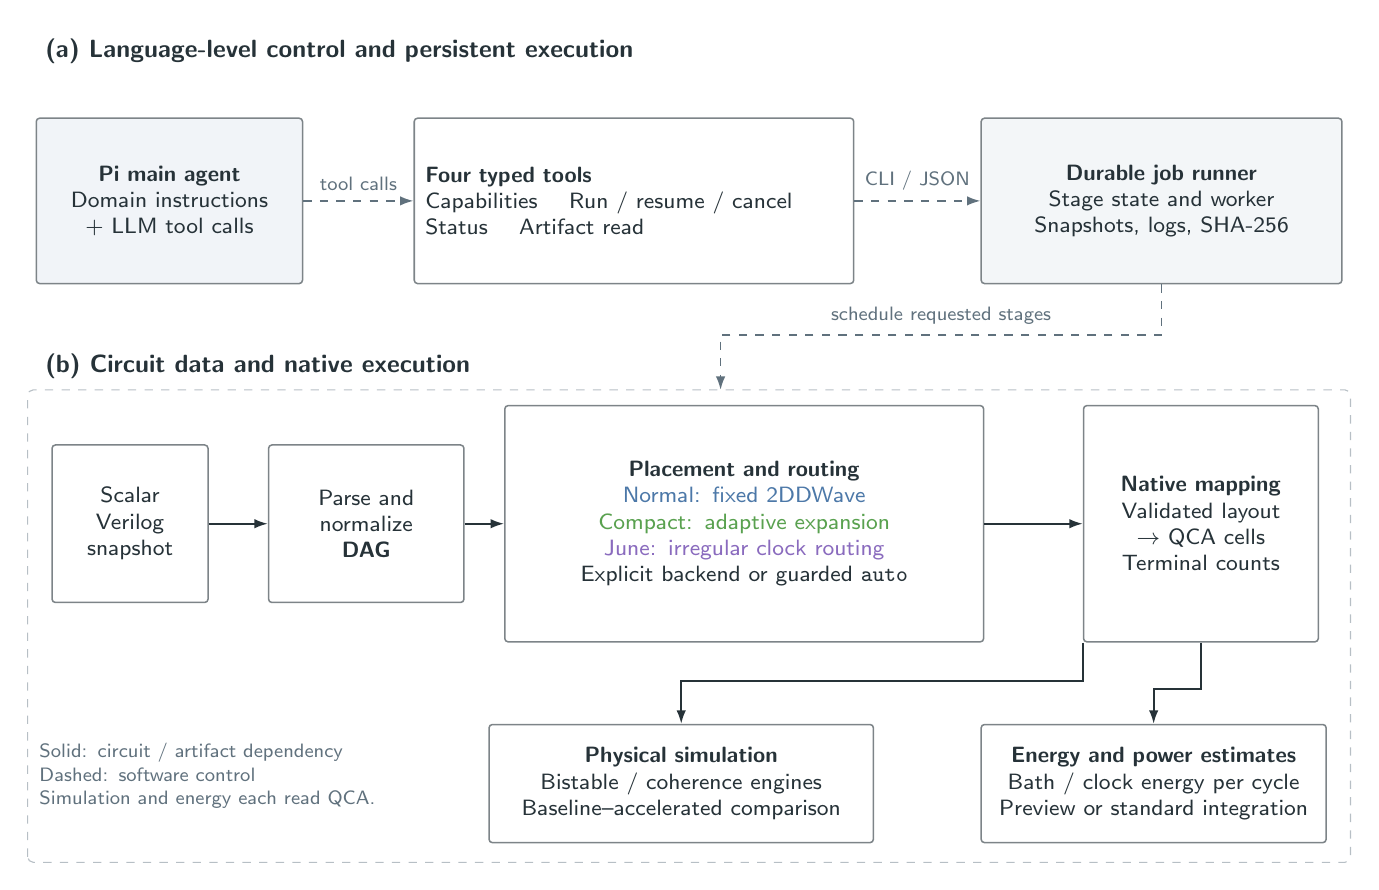
\begin{tikzpicture}[x=1mm,y=1mm]
  \path[use as bounding box] (0,0) rectangle (168,106);
  \node[paneltitle] at (1,103) {(a) Language-level control and persistent execution};
  \node[box,fill=normal!8,text width=31mm,minimum height=21mm] (agent) at (18,84)
    {\textbf{Pi main agent}\\Domain instructions\\+ LLM tool calls};
  \node[box,text width=53mm,minimum height=21mm,align=left] (tools) at (77,84)
    {\textbf{Four typed tools}\\Capabilities \quad Run / resume / cancel\\Status \quad Artifact read};
  \node[box,fill=grid!35,text width=43mm,minimum height=21mm] (job) at (144,84)
    {\textbf{Durable job runner}\\Stage state and worker\\Snapshots, logs, SHA-256};
  \draw[control] (agent.east) -- node[smallnote,above,align=center] {tool calls} (tools.west);
  \draw[control] (tools.east) -- node[smallnote,above,align=center] {CLI / JSON} (job.west);
  \draw[control] (job.south) -- (144,67) -- node[smallnote,above] {schedule requested stages} (88,67) -- (88,60);
  \node[paneltitle] at (1,63) {(b) Circuit data and native execution};
  \node[box,text width=17mm,minimum height=20mm] (rtl) at (13,43)
    {Scalar\\Verilog\\snapshot};
  \node[box,text width=22mm,minimum height=20mm] (dag) at (43,43)
    {Parse and\\normalize\\\textbf{DAG}};
  \node[box,text width=58mm,minimum height=30mm] (pnr) at (91,43)
    {\textbf{Placement and routing}\\
    \textcolor{normal}{Normal: fixed 2DDWave}\\
    \textcolor{compact}{Compact: adaptive expansion}\\
    \textcolor{june}{June: irregular clock routing}\\
    Explicit backend or guarded \texttt{auto}};
  \node[box,text width=27mm,minimum height=30mm] (qca) at (149,43)
    {\textbf{Native mapping}\\Validated layout\\$\rightarrow$ QCA cells\\Terminal counts};
  \draw[flow] (rtl.east) -- (dag.west);
  \draw[flow] (dag.east) -- (pnr.west);
  \draw[flow] (pnr.east) -- (qca.west);
  \node[box,text width=46mm,minimum height=15mm] (sim) at (83,10)
    {\textbf{Physical simulation}\\Bistable / coherence engines\\Baseline--accelerated comparison};
  \node[box,text width=41mm,minimum height=15mm] (energy) at (143,10)
    {\textbf{Energy and power estimates}\\Bath / clock energy per cycle\\Preview or standard integration};
  \draw[flow] (qca.south west) -- (qca.south west |- 0,23) -- (83,23) -- (sim.north);
  \draw[flow] (qca.south) -- (qca.south |- 0,22) -| (energy.north);
  \node[smallnote,text width=47mm] at (25,11)
    {Solid: circuit / artifact dependency\\Dashed: software control\\Simulation and energy each read QCA.};
  \begin{scope}[on background layer]
    \draw[draw=muted!45,dashed,rounded corners=2pt] (0,0) rectangle (168,60);
  \end{scope}
\end{tikzpicture}
\end{document}
